
\newpage
{\bfseries МРНТИ 81.93.29}

\sectionwithauthors{А. Адамова, Т. Жукабаева}{ЗАТТАР ИНТЕРНЕТІ ҚҰРЫЛҒЫЛАРЫНЫҢ ҚАУІПСІЗДІГІН ҰЙЫМДАСТЫРУДА
ФЕДЕРАТИВТІ ОҚЫТУ ӘДІСТЕРІН ҚОЛДАНУ}

\begin{center}

{\bfseries \textsuperscript{1}А. Адамова\textsuperscript{🖂},
\textsuperscript{1,2}Т. Жукабаева}

\textsuperscript{1}Astana IT University, Астана, Қазақстан,

\textsuperscript{2}Л.Н. Гумилев атындағы Еуразиялық ұлттық университеті,
Астана, Қазақстан
\end{center}
Корреспондент-автор:\emph{aigul.adamova@astanait.edu.kz}\vspace{0.5cm}

Заттар интернеті құрылғыларының өзара әрекеттесуінің негізгі
технологияларының бірі болып табылады. Заттар интернеті құрылғыларының
өзара әрекеттесуі кезінде ресурстардың белгілі шектеу-лері бар. Бұл
шектеулер заттар интернеті құрылғыларының нақты уақыт режиміндегі өзара
әрекетте-суіне әсер етеді және желіні пайдаланушылардың жеке деректерінің
қауіпсіздігі мәселесіне әсерін береді. Бұл жұмыс заттар интернеті
құрылғыларының қауіпсіздігін арттыру мақсатында, машиналық оқытудың
иновациялық әдісі болып табылатын -- федеративті оқытудың қолданылуын
зерттеу туралы. Мақалада федеративті оқытудың әлемдік зерттеулерде
қолданылуы туралы шолу келтірілген. Федера-тивті оқытудың ``Federative
average'' әдісі көмегімен тоғыз заттар интернеті құрылғыларының өзара
әрекеттесуі барысында алынған желілік трафик бойынша DDoS щабуылын
анықтау жолы талданған. Нәтижесінде бағалау көрсеткіштері арқылы ұсынған
жүйенің қолданылуы бағаланды.

{\bfseries Түйін сөздер}: Заттар интернеті, қауіпсіздік, желілік шабуылдар,
машиналық оқыту, федеративті оқыту, DDoS


\sectionheading{ОБЕСПЕЧЕНИЕ БЕЗОПАСНОСТИ УСТРОЙСТВ ИНТЕРНЕТ ВЕЩЕЙ С ПОМОЩЬЮ МЕТОДОВ ФЕДЕРАТИВНОГО ОБУЧЕНИЯ}
\begin{center}
{\bfseries \textsuperscript{1}А. Адамова\textsuperscript{🖂},
\textsuperscript{1,2}Т. Жукабаева}

\textsuperscript{1}Astana IT University, Астана, Казахстан,

\textsuperscript{2}Евразийский национальный университет им. Л. Н.
Гумилева, Астана, Казахстан

е-mail: aigul.adamova@astanait.edu.kz
\end{center}

Интернет вещей является одной из основных технологий взаимодействия
устройств. При взаимо-действии устройств Интернета вещей существуют
определенные ограничения ресурсов. Эти ограни-чения влияют на
взаимодействие устройств Интернета вещей в режиме реального времени и
влияют на проблему безопасности личных данных пользователей сети.
Представленная работа посвящена изучению использования федеративного
обучения который является инновационным подходом ма-шинного обучения, с
целью повышения безопасности устройств Интернет вещей. В статье
представ-лен обзор использования федеративного обучения в мировых
исследованиях. С помощью метода федеративного обучения ``Federative
average'' анализируется сетевой трафик, полученный при взаимо-действии
девяти устройств Интернет вещей на выявление DDoS атак. В результате
оценивалось применение предложенной системы с помощью оценочных
показателей.

{\bfseries Ключевые слова:} Интернет вещей, безопасность, сетевые атаки,
машинное обучение, федератив-ное обучение, DDoS атака


\sectionheading{ENSURING THE SECURITY OF INTERNET OF THINGS DEVICES USING FEDERATED LEARNING METHODS}
\begin{center}
{\bfseries \textsuperscript{1}А. Аdamova\textsuperscript{🖂},
\textsuperscript{1,2}Т. Zhukabayeva}

\textsuperscript{1}Astana IT University, Astana, Kazakhstan,

\textsuperscript{2} L.N. Gumilyov Eurasian National University, Astana,
Kazakhstan

е-mail: aigul.adamova@astanait.edu.kz
\end{center}

The Internet of Things (IoT) is one of the key technologies for device
interaction. However, there are certain resource limitations in IoT
device interactions. These limitations impact real-time interactions of
IoT devices and pose challenges to the security of
users\textquotesingle{} personal data within the network. This work
explores the use of federated learning, an innovative machine learning
approach, to enhance the security of IoT devices. The article provides
an overview of the use of federated learning in global research. The
federated learning method \textquotesingle Federated
Average\textquotesingle{} is used to analyze network traffic generated
by the interaction of nine IoT devices to detect DDoS attacks. The
proposed system was evaluated using performan-ce metrics.

{\bfseries Keywords}: Internet of Things, security, network attack,
machine learning, federated learning, DDoS.
\begin{multicols}{2}

{\bfseries Кіріспе.} Қазіргі таңда өнеркәсіптің және адамның күнделікті
қызмет салаларының сандық трансформациялануы, 4.0 Индустриясының,
сенсорлы және пилотсыз технологиялардың дамуы, физикалық үрдістерді
өзара ақпаратпен алмасу арқылы іске асыратын Интернет заттардың
(Internet of Things, IoT) кең таралуына себеп болды. Күн сайын үлкен
көлемдегі деректерді жинауға және тасымалдауға қабілетті жаңа құрылғылар
шығарылуда. IoT құрылғылары түрлі деректерді жинайды, олардың ішінде
жеке ақпарат, құпия немесе қауіпсіздікпен байланысты ақпарат. IoT
құрылғылар санының қарқынды өсуі - ақпараттың қауіпсіздігі мен
құпиялылығына байланысты жаңа мүмкіндіктермен қатар, үлкен қиындықтарды
тудырады. Бұл кеңейіп келе жатқан экожүйенің қауіпсіздігі мен
сенімділігін қамтамасыз ету үшін, бұл мәселелерді түбегейлі шешу қажет.
Үлкен деректер, IoT құрылғыларының алуан түрі көптеген шабуылдарға тап
болуы жаңалық емес. IoT құрылғыларымен жиналатын деректерге рұқсатсыз
қол жеткізу қаржылық шығындарға, физикалық қауіпке және түрлі
зардаптарға әкелуі мүмкін. 2016 жылы қауіпсіздік камерасының белгілі бір
үлгісінде осалдылық табылып, 300 мыңға жуық IoT бейнежазба жүргізетін
құрығылар арқылы Spotify, Reddit сияқты әлеуметтік желілерге шабуылдар
жасалған {[}1{]}. 2019 жылы Wyze Labs Inc. компаниясы ақылды үй
қауіпсіздік жүйесінің бұзылғаны туралы хабарланған, онда 2,4 миллионға
жуық қолданушылардың жеке мәліметтерінің құпиялылығы сақталмаған
{[}2{]}. Онымен қатар, 2024 жылдың ақпан айында Wyze Labs ақылды үйге
арналған камера өндіруші компаниясы өз қолданышуларына қызмет көрсетуін
тоқтатуға мәжбүр болды. 13000 қолданушыға қатысты емес, басқа ақылды
үйлердің бейнежазба деректері келіп түскен. Бұл жағдай желілік
хаттамалар осалдылық салдарынан орын алды {[}3{]}. IoT құрылғыларының
өзара әрекеттесу барысында ақпараттың құпиялылығын сақтау, аталған
жағдайлардың қайталанбауы немесе оларды алдын алу - қазіргі таңда өзекті
мәселелердің бірі болып келеді.

IoT құрылғыларының ақпараттық қауіпсіздігін ұйымдастыру бойынша, бүгінгі
күні, танымал әдістердің негізін құрайтын машиналық оқыту әдістері кең
қолданылуда. IoT қауіпсіздігін ұйымдастыру барысында K-Nearest Neighbor,
Artificial Neural Network, Support Vector Machine, Decision Tree, Random
Forest, Logistic Regression және тағы көптеген машиналық оқытудың
әдістерінің қолданылу аясы ауқымды {[}4{]}. Машиналық оқыту әдістері
жиналған деректерді талдай отырып, қалыпты жағдайдан ауытқуларды нақты
уақыт режимінде анықтап, қауіптерді болжай алады {[}5{]}. Дәстүрлі
Машиналық оқыту әдістері көбінесе орталықтандырылған серверде үлкен
көлемдегі деректерді жинау мен оларды талдау үрдістерін қамтиды
{[}6,7{]}. Дегенмен, бұл тәсіл құпиялылық тұрғысынан деректер
қауіпсіздігінің бұзылуы, жеке деректерді қорғау туралы қатаң заңдардың
болуы, сенімсіздіктің болуы сияқты бірқатар қиындықтарды тудырады.
Ұсынылып отырған мақалада IoT құрылғылар рөлінің артуы, құпия
деректердің маңыздылығына байланысты ақпараттың құпиялылығын сақтауға
және бір уақытта модельдердің жоғары дәлдігін қамтамасыз етуге мүмкіндік
беретін машиналық оқытудың жаңа тәсілі - федеративті оқыту зерттеледі.

Федеративті оқыту - модельді үлестірілген деректер негізінде оқытатын
машиналық оқытудың нновациялық әдісі болып келеді {[}8{]}. Бұл жағдайда
деректер орталық серверде жиналмайды, онымен қоса аталған әдіс -
деректер құпия болған жағдайда аса пайдалы болып келеді {[}9{]}.
Федеративті оқыту негізіндегі әдістер дәстүрлі орталықтандырылған
машиналық оқыту нұсқаларымен салыстырғанда - қолданышулардың жеке
деректерінің құпиялығын сақтауда және шабуылды анықтау нақтылығында
жоғары көрсеткішті шешімдер көрсетеді {[}10{]}. Жеке деректердің
құпиялығы мен жүйенің сенімділігін арттыру мақсатында федеративті
оқытуды блокчейн технологиясымен IoT жүйелерінде аномалияны анықтау үшін
қолданады {[}11{]}. IoT құрылғылары-ның ресурстарының жетіспеушілігі
шектелген есептеу қабілеті, төмен өткізгіштік қабілеті, төмен қуаттылығы
және шектелген жадыға байланысты. осыған байланысты, IoT құрылғыла-ры
үшін үлестірілген машиналық оқыту жолдары қз қолданысын тапқан болатын
{[}12{]}. Сайып келгенде, федеративті оқыту тәсілінің IoT құрылғылары
желісінде жеке деректердің құпиялығын сақтаудағы перспективасы анық.
Жұмыс барысында IoT құрылғылар желісіндегі Ddos шабуылын анықтау үшін
федеративті оқыту әдісі негізіндегі жүйе ұсынылады. Федеративті оқыту
мен деректерді талдау үйлесімі пайдаланушылардың құпиялылығын бұзбай,
DdoS шабуылдарымен тиімді күресуге мүмкіндік береді. Бұл қауіпсіз және
сенімді заттар интернетін дамытудың жаңа мүмкіндікте-рін ашады.

{\bfseries Материалдар мен әдістер.} IoT жүйелерінің дәстүрлі үш деңгейлі
архитектурасы қарастыра-тын болсақ, әрбір деңгейге тән қауіпсіздік
қатерлерін байқауға болады. Қауіпсіздік қатерлері жеке деректердің
бұзылуына әкеледі {[}13{]}. Үш деңгейлі архитектурасы қосымша, желілік
және сенсорлық деңгейлерден тұрады {[}14{]}. Сенсорлы деңгейдегі
шабуылдар рұқсатсыз кіру немесе бақылау үшін, құрылғының
микробағдарламасындағы әлсіз жерлерді пайдалану арқылы, құпия ақпаратты
алу үшін құрылғылардың физикалық сипаттамаларын талдау арқылы,
құрылғыларға рұқсатсыз кіру үшін ұрланған тіркелгі деректерін пайдалану
арқылы, өндіріс процесіне зиянды компоненттерді немесе бағдарламалық
жасақта-маны енгізу арқылы жасала алады {[}15{]}. Желілік деңгейдегі
шабуылдар ретінде құрылғылар мен шлюз арасындағы байланысты ұстап алу
және басқару арқылы асырылатын MITM немесе шлюзді қол жетімсіз ету үшін
трафиктің шамадан тыс жүктелуін атауға болады {[}16{]}. Қосымша
деңгейіндегі шабуылдар ретінде SQL инъекция арқылы шекті деректерге қол
жеткізу сияқты жағдайларды атауға болады {[}17{]}. Барлық шабуылдар IoT
желісіне үлкен қауіп төндіреді. Осы қауіпті алдын алу алу үшін
федеративті оқытудың IoT қауіпсіздігін ұйымдастыру барысында қолданылуы
туралы соңғы жылдары зерттеген жұмыстарға талдау жасалды. Талдау
нәтижесі 1-кестеде ұсынылған.
\end{multicols}

\newpage


\begin{longtable}[H]{|@{}
  >{\raggedright\arraybackslash}p{(\columnwidth - 6\tabcolsep) * \real{0.1156}}|
  >{\raggedright\arraybackslash}p{(\columnwidth - 6\tabcolsep) * \real{0.1094}}|
  >{\raggedright\arraybackslash}p{(\columnwidth - 6\tabcolsep) * \real{0.3812}}|
  >{\raggedright\arraybackslash}p{(\columnwidth - 6\tabcolsep) * \real{0.3938}}@{}|}
\caption*{1-кесте. Федеративті оқытудың IoT қауіпсізідігінде қолданылған
жұмыстарға шолу}\\
\hline
\toprule\noalign{}
Мақала & жылы & Негізгі мазмұны & Федеративті оқытудың қолданылуы \\
\hline
\endfirsthead
\hline
\toprule\noalign{}
Мақала & жылы & Негізгі мазмұны & Федеративті оқытудың қолданылуы \\
\hline
\endhead
\hline

\endlastfoot
{[}18{]} & 2024 & Авторлар қауіпсіз және тиімді IoT жүйелерін құру үшін кванттық есептеулердің, Федеративті оқытудың және 6g желілерінің тұжырымдамалық интеграциясын ұсынған. & Федеративті оқыту IoT құрылғыларына құпиялылықты қорғау үшін орталық серверге деректерді жібермей модельдерді бірлесіп оқытуға мүмкіндік береді. \\
\hline
{[}19{]} & 2024 & Автор түрлі шабуылдарды анықтауда дәстүрлі орталықтандырылған әдістері ауқымды және әртүрлі IoT желілерінде тиімсіз екенін атап, федеративті оқытуға негізделген жаңа тәсіл ұсынған. & Федеративті оқыту конволюциялық нейронды желілерді пайдаланып DDoS шабуылдарды тиімді анықтауға көмектеседі. \\
\hline
{[}20{]} & 2024 & Мақала Машиналық оқыту алгоритмдерін қолдана отырып, IoT құрылғы хосттарындағы түрлі шабуылдардың жіктелуін ұсынады. & Tree decision, Lite Gradient Boost, Xtra Gradient Boost және Random Forest, сияқты Машиналық оқыту алгоритмдерінің ансамбльдері жоғары дәлдікті қамтамасыз етеді. \\
\hline
{[}21{]} & 2020 & Жұмыста федеративті оқыту барысында қауіпсіздік пен сенімділіктің қатерлері зерттеледі & Федеративті оқыту әрбір қолданышуға модельді жергілікті түрде оқытуға мүмкіндік береді және орталықтандырылған серверде жаһандық агрегация жасалады \\
\hline
{[}22{]} & 2022 & Мақалада киберқауіпсіздік бойынша деректер жинағы ұсынылған & Машиналық оқыту әдістерінің тиімділігі федеративті оқыту режимінде бағаланған \\
\hline
{[}23{]} & 2022 & Жұмыста федеративті оқыту негізінде құрастырылған жаңа алгоритм ұсынылған & Федеративті оқытудың негізгі кемшіліктерін зерттейді. \\
\hline
{[}24{]} & 2023 & Жұмыс жоғары дәлдіктегі және деректердің құпиялылығын қорғауды күшейтетін IoT құрылғыларындағы кибершабуылдарды анықтау үшін FL және көп қабатты перцептронды нейрондық желілерді пайдаланатын хост негізіндегі кіруді анықтау жүйесін ұсынады. & Федеративті оқыту IoT құрылғыларының қауіпсіздігін жақсарту үшін қолданылады \\
\hline
{[}25{]} & 2023 & Жұмыстағы ұсынылған әдіс иерархиялық құрылымды, адаптивті деректерді қысу алгоритмін және IoT құрылғылары мен Орталық сервер арасындағы тиімді, қауіпсіз және құпия өзара әрекеттесу үшін SEP-IoT хаттамасын қамтиды & Федеративті оқыту IoT жүйелеріндегі қауіпсіздік пен құпиялылықты арттыру үшін қолданылады \\
\hline
{[}26{]} & 2023 & Мақалада FLIP 4 жергілікті IoT құрылғыларындағы машиналық оқыту үлгілерін оқытуға мүмкіндік беретін әдіс зерттеледі & FLIP 4-федеративті оқытуға негізделген IoT желісіндегі шабуылдарды анықтауға арналған платформа \\
\hline
\end{longtable}

\begin{multicols}{2}

Осы зерттеу бағытындағы 1-кестеде келтірілген мақалаларды талдай отырып,
федеративті оқыту әдісі - деректерді жергілікті құрылғыларда сақтауға,
дәстүрлі машиналық оқытуға тән шығындарды және өнімділік кедергілерін
азайту арқылы IoT құрылғыларының қауіпсіздігін арттыра алатынына көз
жеткізуге болады. Ол сондай-ақ есептеу және желі шығындарын азайтады,
қауіпсіздік пен құпиялылықты арттырады, параллелизацияны пайдаланады
және смарт жүйелердің тұрақтылы-ғын арттырады. Негізі федеративті
оқытудың FedAvg, FedProx сияқты түрлі алгоритмдері бар. Бұл жұмыста
FedAvg (Federated Averaging) алгоритмін IoT құрылғыларымен жиналған
деректер қорында Ddos шабуылдарды анықтау мақсатымен қолданылады. DDoS
шабуылдары компанияның немесе ұйымның беделіне айтарлықтай зиян келтіруі
мүмкін. DDoS шабуылдарының негізгі мақсаты - интернеттегі кез-келген
ресурсты қол жетімсіз ету. Бұл ұйымдар үшін үлкен қаржылық шығындарға
және пайдаланушылар үшін қолайсыздықтарға әкелуі мүмкін.

FedAvg -- федералды оқытудың ең танымал алгоритмдерінің бірі. Бұл әр
құрылғыда жергілікті деректерді сақтай отырып, көптеген құрылғыларда
машиналық оқыту модельдерін оқытуға мүмкіндік береді {[}27{]}. Алгоритм
8 қадамнан тұратын орындалу үрдісі 1-суретте көрсетілген. Алғашқы
қадамында орталық сервер жаһандық модельді инициализацияласа, келесі
оқыту қадамына қатысу үшін қолданушы-лардың ішкі жиыны таңдалады. Бұл
таңдау ерікті немесе стандарттар жиынтығымен анықталады. Кейін таңдалған
қолданушылар жаһандық үлгіні алады. Модель әр клиенттік құрылғыда
жергілікті деректерді қолдана отырып оқытылады. Модельдің өнімділігін
арттыру мақсатында көптеген итерацияларды немесе түрлі уақыт аралықтары
қамтылуы мүмкін. Келесі қадамда, әрбір клиенттен оқытылған жаңа
модельдер орталық серверге жіберліді. Орталық сервер, клиенттерден
алынған модельдерді - модель параметрлерін орташалау арқылы біріктіреді.
Бұл орташалау процесі жаһандық модельдің құпиялығын сақтай отырып,
әртүрлі қоланушылардан алған ақпараттың пайдалылығын қамтамасыз етеді.
Клиентті таңдау және модельді орташалау арасындағы қадамдар қажетті
өнімділік деңгейіне жеткенше дейін қайталана алады.

Алгоритмді Google Colab ортасында Python бағдарламалау тілінде іске асырылды, кодтың үзіндісі 2-суретте көрсетілген.

FedAvg алгортмінің псевдокодындағы \emph{federated\_averagin} функциясы
серверде федеративті орташалау үрдісін орындайды. Федеративті оқытуда
\emph{global\_model} - бастапқы модель ретінде алынып,
\emph{client\_data} әрбір клиенттен түскен деректер тізімі және
\emph{num\_rounds} раунд санын білдіреді. Әрбір таңдалған клиент өз
жергілікті моделін \emph{train\_local\_model} функциясы көмегімен
оқытады. \emph{aggregated\_model} функциясы әр клиенттік модельдің
салмақтарын қосу арқылы біріктіреді.
\end{multicols}

\begin{figure}[H]
	\centering
	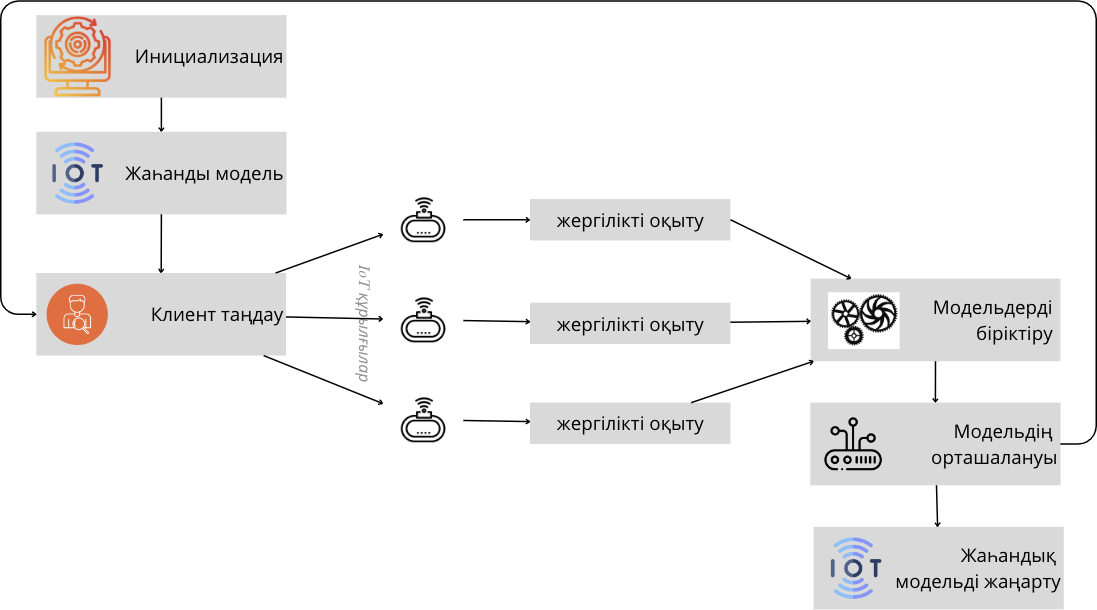
\includegraphics[width=0.7\textwidth]{assets/199}
	\caption*{\bfseries 1-сурет. FedAvg алгортмінің жұмыс істеу қадамдары}
\end{figure}




\begin{figure}[H]
	\centering
	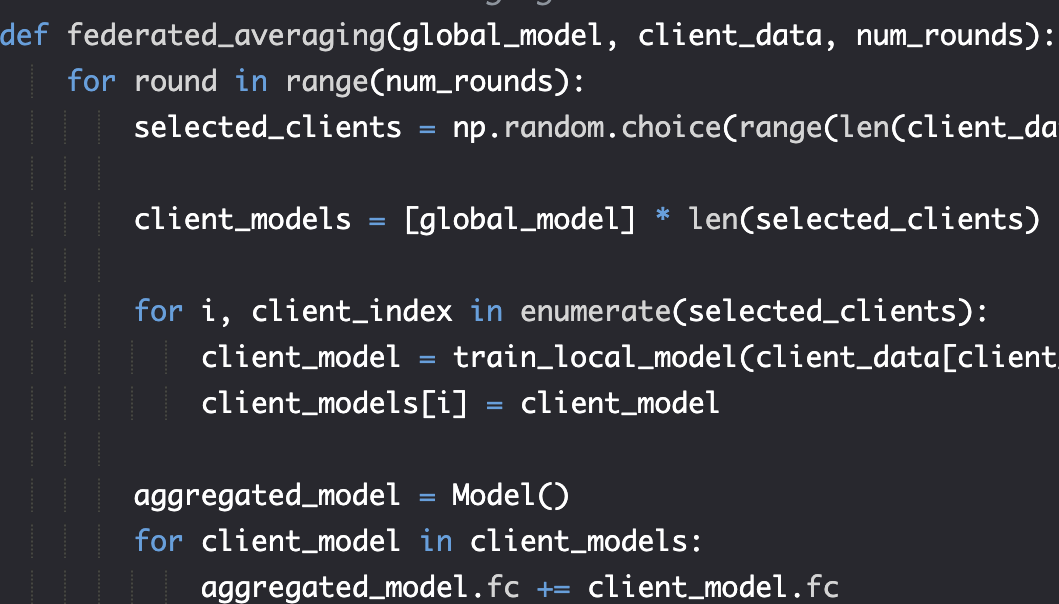
\includegraphics[width=0.6\textwidth]{assets/200}
	\caption*{\bfseries 2-сурет. FedAvg алгортмінің псевдокоды}
\end{figure}


\begin{multicols}{2}


FedAvg - бұл IoT құрылғыларының өзра әрекеттесу барысында құпиялылық
мәселелерін шешудің және машиналық оқытудағы деректерді
орталықсыздандырудың әлеуетті әдісі {[}28{]}. FedAvg деректердің
қауіпсіздігі мен модельдің өнімділігі арасындағы мұқият тепе-теңдікті
қамтамасыз етеді, сонымен бірге пайдаланушы деректерінің құпиялылығын
сақтап, модельдерді белгілі бір құрылғыларда немесе серверлерде
жергілікті түрде оқытуға мүмкіндік береді. Ұсынылып отырған жүйенің
сұлбасы 3-суретте келтірілген.
\end{multicols}

\begin{figure}[H]
	\centering
	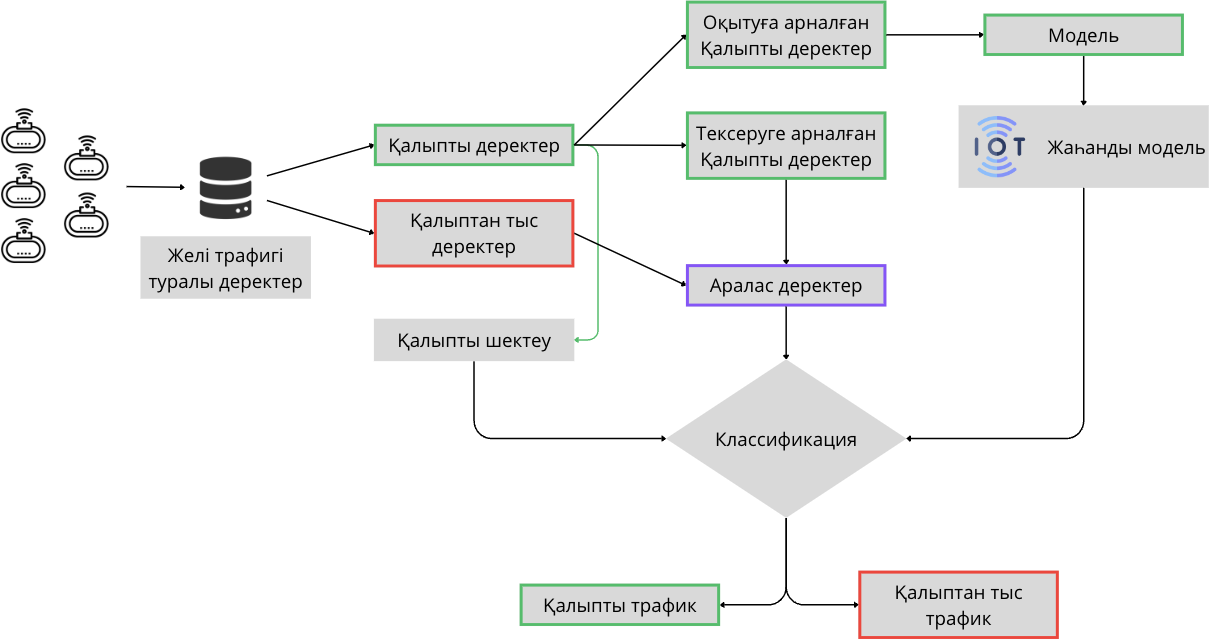
\includegraphics[width=0.7\textwidth]{assets/201}
	\caption*{\bfseries 3-сурет. Ұсынылған жүйе.}
\end{figure}

\begin{multicols}{2}


Осы жұмыста ұсынылған федеративті оқыту әдісі IoT құрылғылар
желілеріндегі DDoS шабуылдар қаншалықты төмендететінін анықтау үшін
Accuracy, Precision және Recall бағалау көрсеткіштері қолданылады.
Accuracy - барлық жағдайлардың дұрыс болжанған мысалдарының пайызын
көрсете отырып, жіктеу нәтижелерінің жалпы дұрыстығын бағалайды.
Precision - модельдің жалған оң нәтижелерді азайту қабілеті туралы
түсінік бере отырып, барлық оң болжамдардың нақты оң болжамдарына үлесін
сандық түрде анықтайтын өлшем. Recall - модельдің шынайы оң жағдайларды
анықтау қабілетін көрсететін барлық нақты оң жағдайлардың шынайы оң
болжамдарының үлесін өлшейді.

{\bfseries Нәтижелер мен талқылау.} Жұмыста зерттелген федеративті оқыту
әдісі DDoS шабуылдарын анықтауда айтарлықтай тиімділік көрсетеді.
Ұсынылған әдістің бағалау өлшемдері-нің көрсеткіштері 2-кесте мен
4-суретте сәйкес келтірілген. Аталған суреттерде 9 IoT құрылғы бойынша
өлшемдер көрсетілген. Нәтижесінде 4a-суретте 3 және 9 құрылғыларды
есептемегенде, алынған модельдің жоғары дәлдігі нақты көрінеді. Орта
есеппен DDOS шабуылын анықтауда алынған модельдің 99,7 \% дұрыс шешімді
болды (Сурет 4b). Модельдің шынайы оң жағдайларды анықтау қабілеті
90,0\% орта көрсеткішке жетті (Сурет 4c).
\end{multicols}

\begin{figure}[H]
  \centering
  \begin{minipage}{0.3\textwidth}
      \centering
      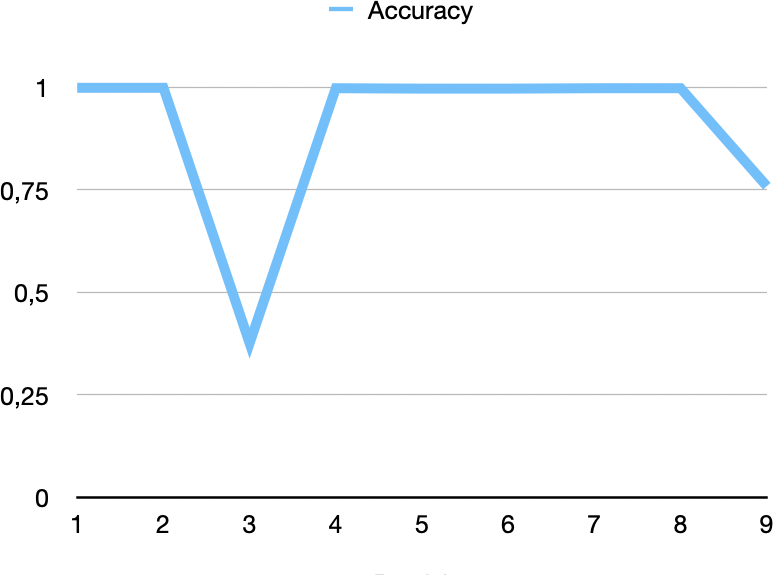
\includegraphics[width=\textwidth]{assets/202}
      \caption*{a) Accuracy}
  \end{minipage}
  \hfill
  \begin{minipage}{0.3\textwidth}
      \centering
      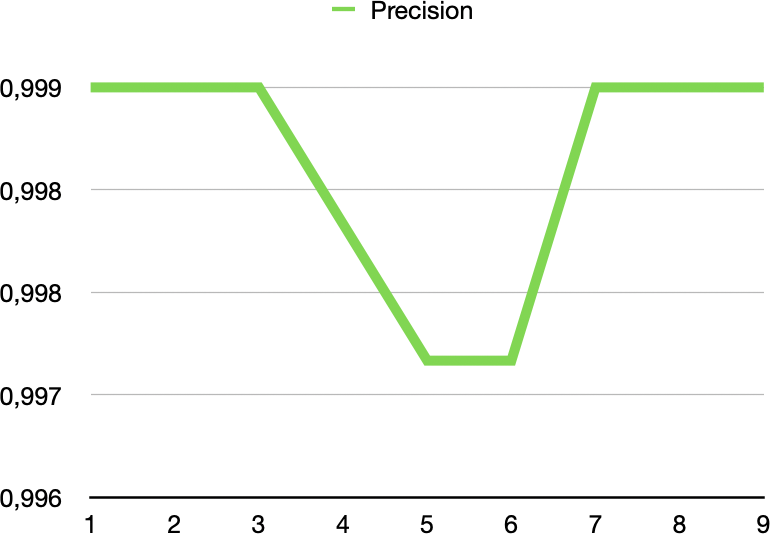
\includegraphics[width=\textwidth]{assets/203}
      \caption*{b) Precision}
  \end{minipage}
  \hfill
  \begin{minipage}{0.3\textwidth}
      \centering
      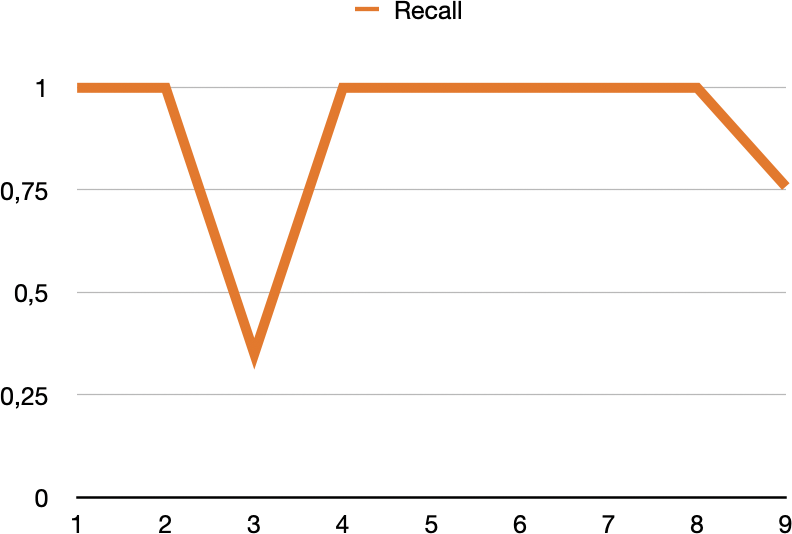
\includegraphics[width=\textwidth]{assets/204}
      \caption*{c) Recall}
  \end{minipage}
  \caption*{\bfseries 4-сурет. Бағалау көрсеткіштерінің құрылғыларға қатысты мәні}
\end{figure}

\begin{multicols}{2}

Fedavg деректерді тарату теңдестірілген желілерде жақсы жұмыс істейтіні
белгілі. Алайда, деректердің таралуы әр түрлі болатын жағдайларда оның
конвергенция проблемалары бар екендігі анықталды. Бұл әдетте федералды
желілерде жиі кездесетін жағдай, мұнда әр клиент өз деректерін
пайдаланады. 2-кестеде Машиналық оқытудың түрлі әдістері көмегімен
алынған бағалау көрсеткіштерінің мәндері келтірілген. Бағалау
көрсеткіштерінің мәні көптеген факторларға тәуелді болып келеді.
Салыстырылған зерттеу жұмыстарында ашық деректер жиындары негізінде
зерттелген әдістердің қорытындысы келтірілген. Осы зерттеуде ұсынылған
жүйенің бағалау мәндері Precision бойынша жоғары көрсеткішті көрсетуде.
Бұл нәтиже федеративті оқытудың қауіпсіздік саласындағы қолданылуының
жаңа мүмкіндіктерінің болуына көз жеткізеді.
\end{multicols}




\begin{longtable}[H]{|@{}
  >{\raggedright\arraybackslash}p{(\columnwidth - 10\tabcolsep) * \real{0.2193}}|
  >{\raggedright\arraybackslash}p{(\columnwidth - 10\tabcolsep) * \real{0.1228}}|
  >{\raggedright\arraybackslash}p{(\columnwidth - 10\tabcolsep) * \real{0.1140}}|
  >{\raggedright\arraybackslash}p{(\columnwidth - 10\tabcolsep) * \real{0.1380}}|
  >{\raggedright\arraybackslash}p{(\columnwidth - 10\tabcolsep) * \real{0.1424}}|
  >{\raggedright\arraybackslash}p{(\columnwidth - 10\tabcolsep) * \real{0.2636}}@{}|}
\caption*{2-кесте. Бағалау көрсеткіштерінің орташа мәні}\\
\hline

Өлшемдер & {[}29{]} & {[}30{]} & {[}31{]} & {[}32{]} & Ұсынылған жүйе \\
\hline
\endfirsthead
\hline
\toprule\noalign{}
Өлшемдер & {[}29{]} & {[}30{]} & {[}31{]} & {[}32{]} & Ұсынылған жүйе \\
\hline
\endhead
\hline
\endlastfoot
Accuracy & 94,02 & 88,76 & - & 97,7 & 90,2 \\
\hline
Precision & 88,77 & 60 & 82 & 97,1 & 99,7 \\
\hline
Recall & 89,23 & 74,36 & 71 & 97,1 & 90,0 \\
\hline
\end{longtable}

\begin{multicols}{2}

{\bfseries Қорытынды.} IoT қауіпсіздік мәселелері көп қырлы және ықтимал
кибершабуылдарды, осалдықтарды және сенімді қауіпсіздік шараларын
қабылдау қажеттілігін
қамтиды.\hspace{0pt}\hspace{0pt}\hspace{0pt}\hspace{0pt}\hspace{0pt}\hspace{0pt}\hspace{0pt}
Машиналық оқыту мен жасанды интеллектті қолдану IoT қауіпсіздігін
жақсартудың перспективалы мүмкіндіктерін ашады, ал ойластырылған
қауіпсіздік және тәуекелге негізделген қауіпсіздік механизмдері сияқты
озық тәжірибелер IoT құрылғылары мен желілерін қорғау үшін өте маңызды.
Ұсынылған жұмыста IoT құрылғыларының өзара байланыс кезінде
қауіпсіздігін арттыру мақстында федеративті оқыту әдісін қолданылу
зерттелген. Тәжірибелік зерттеу барысында 9 IoT құрылғыларының өзара
байланыс кезінде генерацияланған желілік трафик пайдаланып, жаһанды
модельді оқыту әрбір құрылғының жергілікті модельдердің көмегімен
жүргізіліп, ақпаратты жіберу барысында құпиялылықты сақтау және Ddos
шабуылдарын анықтау сұрақтарына назар аударылды. Қорытында федеративті
оқытудың қауіпсіздік деңгейін жаңа деңгейге шығару перспективасы
байқалды. бұл гипотезаны әлі де болашақ жұмыстарда зерттеу көзделуде.

IoT дәуірінде деректердің құпиялылығы барған сайын өзекті мәселеге
айналуда. Деректерді орталықтандырылған жинау және өңдеу ақпараттың ағып
кету қаупін тудырады және пайдаланушылардың құқықтарын бұзады.
Федеративті оқыту деректерді орталықтандырылған сақтаусыз талдауға
мүмкіндік беретін қауіпсіз және сенімді тәсілді ұсынады, бұл құпиялылық
тәуекелдерін айтарлықтай азайтады.

\emph{{\bfseries Қаржыландыру.} Бұл зерттеу Қазақстан Республикасы Ғылым
және жоғары білім министрлігінің Ғылым комитетімен қаржылан-дырған (Грант
NoAP14973006).}
\end{multicols}



\begin{center}
  {\bfseries References}
  \end{center}

\begin{noparindent}

1. Karas B. (2017). Hikvision Backdoor Confirmed. IPVM
https://ipvm.com/reports/hik-backdoor

2. Porter J. (2019) Wyze server leak exposes customer data of 2.4
million users
https://www.theverge.com/\\2019/12/30/21042974/wyze-server-breach-cybersecurity-smart-home-security-camera

3. Cerullo M. (2024) Wyze camera breach may have let 13,000 customers
peek into others\textquotesingle{} homes
\\https://www.cbsnews.com/news/wyze-camera-breach-let-13000-customers-peek-into-others-homes/

4. F. Alwahedi, A. Aldhaheri, M. A. Ferrag, A. Battah, and N. Tihanyi,
Machine learning techniques for IoT security: Current research and
future vision with generative AI and large language models, Internet of
Things and Cyber-Physical Systems, vol. 4, pp. 167--185, 2024, doi:
10.1016/j.iotcps.2023.12.003.

5. M. A. Ferrag et al., ``Edge Learning for 6G-Enabled Internet of
Things: A Comprehensive Survey of Vulnerabilities, Datasets, and
Defenses,'' IEEE Communications Surveys \&amp; Tutorials, vol. 25, no.
4, pp. 2654--2713, 2023, doi: 10.1109/comst.2023.3317242.

6. R. Ahmad and I. Alsmadi, ``Machine learning approaches to IoT
security: A systematic literature review,'' Internet of Things, vol. 14,
p. 100365, Jun. 2021, doi: 10.1016/j.iot.2021.100365.

7. I. H. Sarker, A. I. Khan, Y. B. Abushark, and F. Alsolami, ``Internet
of Things (IoT) Security Intelligence: A Comprehensive Overview, Machine
Learning Solutions and Research Directions,'' Mobile Networks and
Applications, vol. 28, no. 1, pp. 296--312, Mar. 2022, doi:
10.1007/s11036-022-01937-3.

8. B. Ghimire and D. B. Rawat, ``Recent Advances on Federated Learning
for Cybersecurity and Cybersecu-rity for Federated Learning for Internet
of Things,'' IEEE Internet of Things Journal, vol. 9, no. 11, pp.
8229--8249, Jun. 2022, doi: 10.1109/jiot.2022.3150363.

9. L. U. Khan, W. Saad, Z. Han, E. Hossain, and C. S. Hong, ``Federated
Learning for Internet of Things: Recent Advances, Taxonomy, and Open
Challenges,'' IEEE Communications Surveys \&amp; Tutorials, vol. 23, no.
3, pp. 1759--1799, 2021, doi: 10.1109/comst.2021.3090430.

10. V. Mothukuri, P. Khare, R. M. Parizi, S. Pouriyeh, A. Dehghantanha,
and G. Srivastava, ``Federated-Learning-Based Anomaly Detection for IoT
Security Attacks,'' IEEE Internet of Things Journal, vol. 9, no. 4, pp.
2545--2554, Feb. 2022, doi: 10.1109/jiot.2021.3077803.

11. D. C. Nguyen, M. Ding, P. N. Pathirana, A. Seneviratne, J. Li, and
H. Vincent Poor, ``Federated Learning for Internet of Things: A
Comprehensive Survey,'' IEEE Communications Surveys \&amp;\\Tutorials,
vol. 23, no. 3, pp. 1622--1658, 2021, doi: 10.1109/comst.2021.3075439.

12. A. Imteaj, U. Thakker, S. Wang, J. Li, and M. H. Amini, ``A Survey
on Federated Learning for Resource-Constrained IoT Devices,'' IEEE
Internet of Things Journal, vol. 9, no. 1, pp. 1--24, Jan. 2022, doi:
10.1109/jiot.2021.3095077.

13. B. Breve, G. Cimino, and V. Deufemia, ``Identifying Security and
Privacy Violation Rules in Trigger-Action IoT Platforms With NLP
Models,'' IEEE Internet of Things Journal, vol. 10, no. 6, pp.
5607--5622, Mar. 2023, doi: 10.1109/jiot.2022.3222615.

14. N. Batra and S. Goyal, ``IoT architecture,'' IoT Fundamentals with a
Practical Approach, pp. 17--70, Jul. 2024, doi: 10.1201/9781003307488-2.

15. G. Sharma, S. Vidalis, N. Anand, C. Menon, and S. Kumar, ``A Survey
on Layer-Wise Security Attacks in IoT: Attacks, Countermeasures, and
Open-Issues,'' Electronics, vol. 10, no. 19, p. 2365, Sep. 2021, doi:
10.3390/electronics10192365.

16. M. Panoff, R. G. Dutta, Y. Hu, K. Yang, and Y. Jin, ``On Sensor
Security in the Era of IoT and CPS,'' SN Computer Science, vol. 2, no.
1, Jan. 2021, doi: 10.1007/s42979-020-00423-5.

17. G. M and P. H B, ``Semantic Query-Featured Ensemble Learning Model
for SQL-Injection Attack Detection in IoT-Ecosystems,'' IEEE
Transactions on Reliability, vol. 71, no. 2, pp. 1057--1074, Jun. 2022,
doi: 10.1109/tr.2021.3124331.

18. D. Javeed, M. S. Saeed, I. Ahmad, M. Adil, P. Kumar, and A. K. M. N.
Islam, ``Quantum-Empowered Federated Learning and 6G Wireless Networks
for IoT Security: Concept, Challenges and Future Directions,'' Dec.
2023, doi: 10.36227/techrxiv.170259169.96559894/v1.

19. Y. Alhasawi and S. Alghamdi, ``Federated Learning for Decentralized
DDoS Attack Detection in IoT Networks,'' IEEE Access, vol. 12, pp.
42357--42368, 2024, doi: 10.1109/access.2024.3378727

20. M. Asad, A. Moustafa, and C. Yu, ``A Critical Evaluation of Privacy
and Security Threats in Federated Learning,'' Sensors, vol. 20, no. 24,
p. 7182, Dec. 2020, doi: 10.3390/s20247182.

21. Granell, C., Kamilaris, A., Kotsev, A., Ostermann, F.O., Trilles, S.
(2020). Internet of Things. In: Guo, H., Goodchild, M.F., Annoni, A.
(eds) Manual of Digital Earth. Springer, Singapore.
\\https://doi.org/10.1007/978-981-32-9915-3\_11

22. Ferrag, M. A., Friha, O., Hamouda, D., Maglaras, L., \& Janicke, H.
(2022). Edge-IIoTset: A new comprehensive realistic cyber security
dataset of IoT and IIoT applications for centralized and federated
learning. IEEE Access, 10, 40281-40306.
DOI:10.36227/techrxiv.18857336.v1

23. S. Tabatabai et al., ``Exploration and Exploitation in Federated
Learning to Exclude Clients with Poisoned Data,'' 2022 International
Wireless Communications and Mobile Computing (IWCMC), May 2022, doi:
10.1109/iwcmc55113.2022.9825004.

24. V. Holubenko, P. Silva, and C. Bento, ``An Intelligent Mechanism for
Monitoring and Detecting Intrusions in IoT Devices,'' 2023 IEEE 20th
Consumer Communications \&amp; Networking Conference (CCNC), Jan. 2023,
doi: 10.1109/ccnc51644.2023.10060443.

25. K. A. Awan, I. U. Din, A. Almogren, and J. J. P. C. Rodrigues,
``Privacy-Preserving Big Data Security for IoT With Federated Learning
and Cryptography,'' IEEE Access, vol. 11, pp. 120918--120934, 2023, doi:
10.1109/access.2023.3328310.

26. M. Zang, C. Zheng, T. Koziak, N. Zilberman, and L. Dittmann,
``Federated Learning-Based In-Network Traffic Analysis on IoT Edge,''
2023 IFIP Networking Conference (IFIP Networking), Jun. 2023, doi:
10.23919/ifipnetworking57963.2023.10186438.

27. J. Mills, J. Hu, and G. Min, ``Communication-Efficient Federated
Learning for Wireless Edge Intelligen-ce in IoT,'' IEEE Internet of
Things Journal, vol. 7, no. 7, pp. 5986--5994, Jul. 2020, doi:
10.1109/jiot.2019.\\2956615.

28. L. Almeida, P. Rodrigues, R. Teixeira, M. Antunes, and R. L. Aguiar,
``Privacy-Preserving Defense: Intrusion Detection in IoT using Federated
Learning,'' 2024 IEEE 22nd Mediterranean Electrotechnical Conference
(MELECON), Jun. 2024, doi: 10.1109/melecon56669.2024.10608461.

29. M. AlJamal, A. Mughaid, B. Al shboul, H. Bani-Salameh, S. Alzubi,
and L. Abualigah, ``Optimizing risk mitigation: A simulation-based model
for detecting fake IoT clients in smart city environments,'' Sustainable
Computing: Informatics and Systems, vol. 43, p. 101019, Sep. 2024, doi:
10.1016/j.suscom.\\2024.101019.

30. A. R. Kairaldeen, N. F. Abdullah, A. Abu-Samah, and R. Nordin,
``Peer-to-Peer User Identity Verifica-tion Time Optimization in IoT
Blockchain Network,'' Sensors, vol. 23, no. 4, p. 2106, Feb. 2023, doi:
10.3390/s23042106.

31. P. Dey, S. K. Chaulya, and S. Kumar, ``Secure decision tree twin
support vector machine training and classification process for encrypted
\textless scp\textgreater IoT\textless/scp\textgreater{} data via
blockchain platform,'' Concurrency and Computation: Practice and
Experience, vol. 33, no. 16, Mar. 2021, doi: 10.1002/cpe.6264.

32. N. Hasan, Z. Chen, C. Zhao, Y. Zhu, and C. Liu, ``IoT Botnet
Detection framework from Network Behavior based on Extreme Learning
Machine,'' IEEE INFOCOM 2022 - IEEE Conference on Computer
Communications Workshops (INFOCOM WKSHPS), May 2022, doi:
10.1109/infocomwkshps54753.\\2022.9798307.
\end{noparindent}

\emph{{\bfseries Авторлар туралы мәліметтер}}
\begin{noparindent}

Адамова А. - PhD, Astana IT University, Астана, Қазақстан, e-mail:
aigul.adamova@astanait.edu.kz;

Жукабаева Т.К. - PhD, профессор, Л.Н. Гумилев атындағы Еуразия Ұлттық
университеті, Астана, Қазақстан, e-mail: tamarakokenovna@gmail.com
\end{noparindent}

\emph{{\bfseries Information about the authors}}
\begin{noparindent}

Adamova А. - PhD, Astana IT University, Astana, Kazakhstan, e-mail:
aigul.adamova@astanait.edu.kz;

Zhukabayeva Т.К. - PhD, Professor, L. Gumilev Eurasian National
University, Astana, Kazakhstan,\\e-mail: tamarakokenovna@gmail.com
\end{noparindent}





